\chapter{Introduzione alla sicurezza informatica}


\section{Premessa}

\subsection{Definizione}
Che cosa significa sicuro? La parola sicurezza e l’aggettivo sicuro vengono sempre associati a beni che si desidera proteggere da possibili danni, danneggiamenti, perdita, e via dicendo. In particolare un bene è al sicuro se è ben protetto, e la sua messa in sicurezza non deve impedirne l'utilizzo. Esistono molteplici definizioni di sicurezza informatica, ad esempio:
\begin{itemize} 
  \item Security is the degree of protection against danger, damage, loss, and criminal activity ~\cite{wikiSecurity}.
  \item Security is a form of protection where a separation is created between the assets and the threat ~\cite{isecomSecurity}.
\end{itemize}
La parola sicurezza deriva dal latino sine cura: senza preoccupazione. La sicurezza di un sistema può essere definita come la conoscenza del fatto che l’evoluzione del sistema non produrrà stati indesiderati. Le cause che possono minare la sicurezza sono molteplici e spesso
non prevedibili, quindi non si può parlare di sicurezza in senso assoluto, ma solo relativo (\textit{"L'unico computer sicuro è un computer spento"}).

\textbf{Trasversalità della tematica:} Le problematiche di sicurezza interessano molteplici campi (attività lavorative, vita domestica, hobby, giochi, sport, etc.). Di fatto, ogni settore della vita moderna ha delle implicazioni relative alla sicurezza. Il livello di sicurezza di un'organizzazione dipende dai livelli di sicurezza di tutti i suoi comparti/settori. Il livello di sicurezza di un sistema è determinato dal livello di sicurezza dal suo comparto meno sicuro (principio dell'anello debole).


\section{Concetti fondamentali}

\subsection{Sistema informativo e informatico}
\begin{itemize} 
  \item Per sistema informativo (information system) di un’organizzazione si intende l’insieme delle informazioni prodotte ed elaborate e delle risorse umane, materiali e immateriali, coinvolte nel processo di elaborazione di tali informazioni
  \item Per sistema informatico (information and communication technology system) s'intende l'insieme delle varie tecnologie coinvolte nel sistema informativo (il sistema informativo è parte del sistema informatico).
\end{itemize}
Questo corso verterà sulla sicurezza dei sistemi informativi. Tuttavia, si approfondiranno maggiormente questioni inerenti la sicurezza
dei sistemi informatici. Per sicurezza di un sistema informativo si intende il grado di protezione contro qualsiasi minaccia ai suoi asset.
Richiede il soddisfacimento dei seguenti requisiti:
\begin{itemize} 
  \item \textbf{confidenzialità, integrità e disponibilità}
  \item \textbf{assicurazione, autenticità e anonimato}
\end{itemize}
Quando si parla di \textbf{attacco} solitamente si intende la violazione di uno o più di questi requisiti.

\subsection{Vulnerabilità, Minacce, Attacchi, Difesa}
\subsubsection{Vulnerabilità}
Una vulnerabilità (o falla o breccia) è una \textbf{debolezza intrinseca} di un sistema, che potrebbe essere sfruttata per provocare perdite o danni. Scaturisce spesso da errate procedure di sicurezza e/o da errori di progettazione/implementazione, e  in alcuni casi è intimamente legata alla natura del sistema. Ad esempio:
\begin{itemize} 
  \item un sistema potrebbe essere vulnerabile alla manipolazione non autorizzata dei dati causa un bug nella procedura di autenticazione dell’utente
  \item un calcolatore è vulnerabile all'acqua
\end{itemize}
Nel primo caso (vulnerabilità scaturite da errate procedure di sicurezza) l'insorgenza delle vulnerabilità può essere mitigata adottando adeguati standard e norme di qualità.

\subsubsection{Minacce (Threats)}
Per minaccia (threat) ad un sistema informatico/informativo si intende quell’insieme di circostanze che potrebbero arrecare danni ai suoi asset: eventi potenziali, accidentali o deliberati, che, nel caso accadessero, produrrebbero perdite e danni. il realizzarsi di una minaccia generalmente avviene sfruttando una o più vulnerabilità del sistema.  Si parla quindi di situazioni ipotetiche che potrebbero avvenire in determinate circostanze. Ad esempio:
\begin{itemize} 
  \item esecuzione di codice malevole che invia dati sensibili ad un'organizzazione criminale
  \item accesso a dati riservati da parte di entità non autorizzate
  \item perdita di dati a causa della rottura di un apparato hardware o al crash di uno specifico software
\end{itemize}

\subsubsection{Attacchi (Attacks)}
Un attacco (attack) è un atto deliberato teso ad arrecare un danno al sistema. Consiste, di fatto, nella realizzazione di una \textbf{minaccia}. Generalmente, un attacco viene perpetrato attraverso lo sfruttamento di una o più vulnerabilità. Spesso si classificano in base all’entità del danno:
\begin{itemize} 
  \item \textbf{attacco attivo (active attack)}: altera le risorse o ne modifica il processo di gestione/elaborazione
  \item \textbf{attacco passivo (passive attack)}: ottiene le informazioni/dati senza alterarli e senza modificare il relativo processo di
gestione/elaborazione
\end{itemize}
Un’altra importante classificazione è in base "al luogo" da cui viene iniziato l’attacco:
\begin{itemize} 
  \item \textbf{attacco dall’interno (inside attack)}: attacco iniziato da un'entità all’interno del perimetro di sicurezza di un sistema informativo di una data organizzazione
  \item \textbf{attacco dall’esterno (outside attack)}: attacco iniziato da un'entità all’esterno del perimetro di sicurezza
\end{itemize}
Ovviamente, è molto più difficile prevenire e rilevare gli attacchi interni di quelli esterni. Ciò anche a causa del fatto che le misure di prevenzione per questo tipo di attacchi limita notevolmente l'usabilità del sistema (si pensi, ad esempio, alla struttura gerachica in ambiente militare, in cui ogni risorsa conosce il minimo indispensabile per svolgere i propri compiti. In questo modo nel caso la risorsa venga compromessa, si limita il danno. Ovviamente tutto ciò rallenta il processo di funzionamento del sistema).

\subsubsection{Tecniche di difesa}
Diverse contromisure (o misure protettive) possono essere attuate per proteggere un sistema informativo da eventi accidentali e da
attacchi deliberati. Tali misure devono essere strutturate all’interno di un piano di sicurezza redatto dopo un’attenta analisi costi/benefici (textit{cost-effective solutions}).
Le tecniche di difesa possono essere di tipo:
\begin{itemize} 
  \item \textbf{preventivo}: effettuano una serie di \textbf{controlli} per evitare \textbf{a priori} che attacchi noti o immaginabili possano essere sferrati con successo (e.g. controlli aeroportuali, controllo di accessi e permessi negli OS).
  \item \textbf{a posteriori}: sono tese a ridurre gli effetti di un attacco che è riuscito a eludere le misure preventive di cui sopra; devono monitorare un sistema ed essere in grado di \textbf{rivelare} comportamenti anomali.
\end{itemize}

Un \textbf{meccanismo di sicurezza} è un qualsiasi metodo, strumento, o procedura teso a rilevare, prevenire o porre rimedio agli effetti di un attacco alla sicurezza del sistema. La strategia di difesa, qualunque essa sia, combina in modo opportuno
uno o più meccanismi di sicurezza. molti meccanismi di sicurezza consistono in controlli hardware/software.

\subsection{Sicurezza informatica: definizione classica e requisiti CIA}
La sicurezza informatica si fonda sulla protezione dei seguenti macro-requisiti di un sistema informativo (informatico):
\begin{itemize} 
  \item \textbf{Confidenzialità (Confidentiality)}
  \item \textbf{Integrità (Integrity)}
  \item \textbf{Disponibilità (Availability)}
\end{itemize}
Spesso si utilizza l’acronimo C.I.A. per denotarli in modo compatto.
\begin{figure}[htbp]
	\centering%
	\subfigure%
	{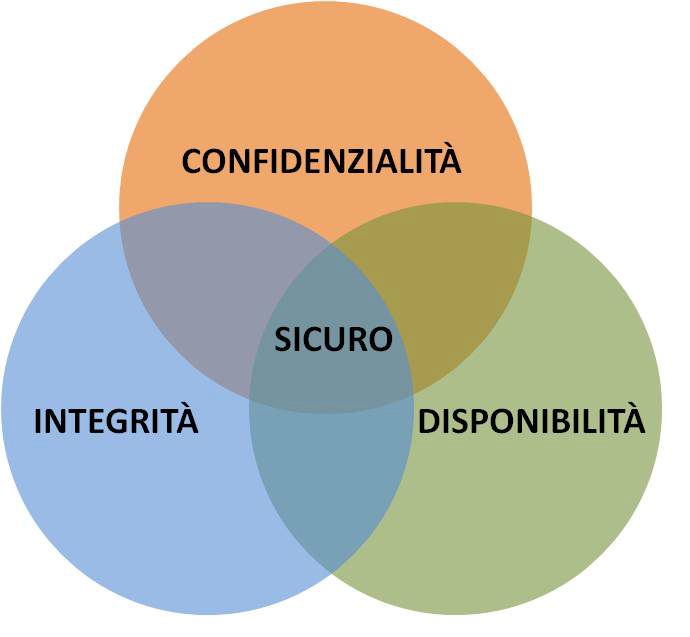
\includegraphics[height=7cm, width=7cm, keepaspectratio]{Immagini/Capitolo1/venn_security}}
	\caption{Diagramma di Venn dei macro-requisiti di sicurezza \label{fig:venn_security}} 	
\end{figure}
Ovviamente, come si può notare dal diagramma di Venn in \figurename ~\ref{fig:venn_security} spesso vengono richiesti contemporaneamente più di questi requisiti, cosi come un attacco può violare più requisiti.

\subsubsection{Confidenzialità (Confidentiality)}
Def. \textbf{Confidentiality}: the property that information is not made available or disclosed to unauthorized individuals, entities, or processes. Per confidenzialità si intende quindi la garanzia che alle risorse informatiche accedano solo le parti autorizzate ad accedervi. E' talvolta denominata segretezza, riservatezza o privacy. Nota bene: per accesso non si intende solo la lettura, ma anche la visualizzazione, la stampa o la semplice consapevolezza dell’esistenza di una data risorsa nel sistema.\newline

\textbf{Attacchi alla confidenzialità:} Si ha un attacco alla confidenzialità quando una entità (persona, processo o risorsa) tenta di accedere senza autorizzazione a informazioni protette (mentre queste sono memorizzate, oppure durante l’elaborazione, oppure ancora durante una comunicazione). La protezione della confidenzialità avviene utilizzando in modo appropriato i seguenti strumenti (meccanismi) di sicurezza informatica:
\begin{itemize} 
  \item \textbf{Cifratura (Encryption)}
  \item \textbf{Controllo degli accessi (Access Control)}
  \item \textbf{Sicurezza fisica (Physical security)}
\end{itemize}

\subsubsection{Integrità (Integrity)}
 Def. \textbf{Integrity}: safeguarding the accuracy and completeness of information and processing methods.\newline
 Def. \textbf{Integrity}: the property of safeguarding the accuracy and completeness of assets.\newline


Per integrità si intende quindi la garanzia che le risorse possano essere modificate solo dalle parti autorizzate e solo nei modi prestabiliti. Le modifiche comprendono la scrittura, la variazione, il cambiamento dello stato, l’eliminazione e la creazione. Nel caso di file, conviene includere anche i metadati associati (proprietario, ultimo utente ad averlo letto, data ultima modifica,data di creazione), in modo che un accesso non autorizzato al contenuto possa essere rivelato da un controllo di integrità applicato ai metadati.\newline

\textbf{Attacchi all'integrità:} Si ha un attacco all'integrità quando una entità (persona, processo o risorsa) tenta di modificare senza autorizzazione una o più risorse del sistema informativo.

 La protezione della confidenzialità avviene utilizzando in modo appropriato i seguenti strumenti (meccanismi) di sicurezza informatica (tutti basati su un uso corretto della ridondanza):
\begin{itemize} 
  \item \textbf{Backup}
  \item \textbf{Somma di controllo o Checksum}
  \item \textbf{Codici a correzione di errore (Corruzioni non deliberate ma accidentali, possono essere facilmente elusi da attacchi intelligenti)}
  \item \textbf{Codici di autenticazione dei messaggi o Message Authentication Code MAC} 
\end{itemize}


\subsubsection{Disponibilità (Availability)}
 Def. \textbf{Availability}: ensuring that authorized users have access to information and associated assets when required. \newline

Per disponibilità (availability) si intende quindi che le risorse siano accessibili, nei tempi e nei modi prestabiliti, alle parti autorizzate ogni volta che le richiedono: se una persona o un sistema dispone dei diritti di accesso ad una risorsa, l’accesso non deve essergli impedito. Spesso la disponibilità viene citata tramite il suo opposto: la \textbf{negazione di servizio} (\textbf{Denial of Service} o \textbf{DoS}). La disponibilità può assumere significati/sfumature diverse; una risorsa può trovarsi in uno stato intermedio tra i due opposti stati di piena disponibilità e di piena indisponibilità.

\subsection{Conflittualità requisiti CIA}

\subsection{Requisiti AAA}

\subsubsection{Assicurazione (Assurance)}

\subsubsection{Autenticità (Authenticity)}

\subsubsection{Anonimato (Anonymity)}

\subsection{Tipologie di Minacce e Attacchi}

\subsubsection{Intercettazione (Eavesdropping)}

\subsubsection{Alterazione (Alteration)}

\subsubsection{Interruzione (Denial-of-service)}

\subsubsection{Falsificazione (Masquerading)}

\subsubsection{Ripudio (Ripudiation)}

\subsubsection{Inferenza (Inference), Correlation and traceback}
Per inferenza o attacco inferenziale si intendono un insieme di tecniche che utilizzando la statistica e l’algebra permettono di ricavare/stimare \textbf{informazioni sensibili} a partire da dati non sensibili. Rappresenta un attacco alla confidenzialità, e spesso è attuato nel contesto dei databases. Similmente, per correlation and traceback si intendono un insieme di tecniche basate sulla statistica e sull’algebra che permettono di determinare la sorgente di una particolare informazione o di un particolare flusso di dati.\newline \newline
\textbf{N.B.:} C'è una differenza, in senso giuridico, tra dati personali e dati sensibili. Tale distinzione dipende dalla giurisdizione dei paesi. In particolare in Italia il dato personale viene indicato come un'informazione che permette di identificare un individuo (anagrafica), mentre un dato sensibile rappresenta un'informazione su aspetti della vita privata dell'individuo (orientamento sessuale, opinione politica, credo religioso, etc.)

\subsection{Principi della Sicurezza Informatica}

\subsubsection{Mediazione completa (Complete mediation):} Ogni accesso ad una risorsa deve essere controllato verificando che sia conforme alle politiche di sicurezza stabilite; diffidare da miglioramenti nell’efficienza ottenuti salvando autorizzazioni precedentemente acquisite, poiché i permessi possono variare nel tempo.

\subsubsection{Struttura aperta (Open design):}  L’architettura, il progetto e l'implementazione dei meccanismi di sicurezza di un sistema devono essere resi pubblici.
\begin{itemize} 
  \item la sicurezza deve fondarsi sulla segretezza di pochi elementi chiave
  \item maggior feedback favoriscono l’individuazione di bug, falle e vulnerabilità, aumentando la robustezza e la sicurezza del sistema
  \item un meccanismo di protezione ritenuto sicuro da molti è preferibile ad uno noto solo a pochi. E' quindi bene evitare meccanismi di sicurezza basati sulla segretezza (security by obscurity).
\end{itemize}

\subsubsection{Separazione dei privilegi (Separation of privilege):} Più condizioni dovrebbero essere richieste per concedere l’accesso a risorse limitate o ottenere il permesso di effettuare una data azione. In genere questo principio comporta una separazione logico/funzionale delle componenti di un sistema.

\subsubsection{Minimo privilegio (Least privilege):} Ogni parte di un sistema deve avere i privilegi minimi necessari allo svolgimento dei propri compiti. Per attività inusuali che richiedono maggiori privilegi conviene assegnare autorizzazioni temporanee fortemente limitate nel tempo. In questo modo si riduce il rischio di attacchi basati sulla scalata di privilegi.

\subsubsection{Minimo meccanismo comune (Least common mechanism):} I meccanismi di sicurezza che per l’accesso e la gestione di risorse condivise non dovrebbero essere a loro volta condivisi o dovrebbero essere condivisi il meno possibile. E' quindi buona norma adottare tecniche di isolamento quali la virtualizzazione e il sandboxing (e.g. browser web: nessuna applicazione web può agire sul filesystem, eccetto attraverso i cookies). In questo modo vengono mitigati rischi derivanti da comportamenti malevoli di utenti cui spetta comunque l’accesso a una data risorsa condivisa.

\subsubsection{Usabilità (Usability, Psychological acceptability):} 

\section{Fondamenti di Crittografia}